\documentclass[xcolor=dvipsnames]{beamer}

\usepackage[english]{babel}
\usepackage[latin1]{inputenc}
\usepackage[T1]{fontenc}

% --- Graphics inclusion.
\usepackage{graphicx}
%\usepackage{float}
%\usepackage{subfigure}
%\usepackage[all]{xy}
\usepackage{caption}

% --- Listing inclusion.
% \usepackage{dsfont}
\usepackage{listings}
% \lstset{numbers=left, numberstyle=\tiny, numbersep=5pt}
% \lstset{language=C}

% --- Verbatim file inclusion.
%\usepackage{verbatim} % include entire files verbatim, \verbatiminput{...}

% --- Indent verbatim environments
\makeatletter \def\verbatim@startline{\verbatim@line{\leavevmode\kern20pt\relax}} \makeatother

% --- Color names.
%\usepackage{color}
%\usepackage[usenames,dvipsnames]{xcolor}
%\usepackage[svgnames]{xcolor}
% Define user colors using the RGB model
%\definecolor{darkgrey}{rgb}{0.8,0.8,0.8}
%\definecolor{lightgrey}{rgb}{0.95,0.95,0.95}
\definecolor{highlight}{named}{NavyBlue}

% --- Table mashups.
%\usepackage{colortbl}
%\usepackage{tabularx}
%\usepackage{longtable}
%\renewcommand*\arraystretch{2.0}

% --- Clubs and widows.
\clubpenalty = 10000
\widowpenalty = 10000
\displaywidowpenalty = 10000

% --- Vector fonts.
%\usepackage{mathptmx}
%\usepackage[scaled=.90]{helvet}
%\usepackage{courier}
%\usepackage{times} % True Type for normal text
%\usepackage{mathptmx} % True Type for maths

% --- Misc.
%\usepackage{trfrac}   % frac-like lines that are no fractions.
%\usepackage{moreverb} % More fun with {verbatim}
%\usepackage{amsfonts} % mathbb{N} and similar symbols
\usepackage{amsmath}  % \overset
\usepackage{amssymb}  % \ltimes
%\usepackage{pxfonts}  % \lJoin etc.; TypeSystems
%\setcounter{secnumdepth}{3}
%\setcounter{tocdepth}{3}
\usepackage{lastpage}
\usepackage{pifont}

%% Drawing trees and other stuff
\usepackage{tikz}
\usetikzlibrary{trees,arrows}
\usepackage{amssymb}

\let\tikzsquare\square
\renewcommand{\square}{\ensuremath\tikzsquare}

\definecolor{cffffff}{RGB}{255,255,255}
\definecolor{c787aff}{RGB}{120,122,255}
\definecolor{cff7374}{RGB}{255,115,116}
\definecolor{c79ff79}{RGB}{121,255,121}
\definecolor{cff7374}{RGB}{255,115,116}
\definecolor{c7372ff}{RGB}{115,114,255}
\definecolor{c63ff63}{RGB}{99,255,99}
\definecolor{c6365ff}{RGB}{99,101,255}
\definecolor{darkgreen}{RGB}{0,162,0}
\definecolor{darkred}{RGB}{162,0,0}


%% Ticks
\usepackage{pifont}
\newcommand{\tick}{{\color{darkgreen}\checkmark\ }}
\newcommand{\cross}{{\color{darkred}\hspace{1pt}\ding{55}\ }}

%% Checklist
\newcommand{\checklist}[3]{
  \begin{block}{Checklist}
    \centering
    \footnotesize{
      \ifnum#1=0 \cross \else \tick \fi Low avg. path length
      \ifnum#2=0 \cross \else \tick \fi High clustering
      \ifnum#3=0 \cross \else \tick \fi Scale-free degree distribution
    }
  \end{block}
}

\newcommand{\Therefore}{\ensuremath{\Rightarrow} }


% ----- BEAMER SPECIFIC -----


% --- Pretty much the usual beamer theme.
\usepackage{beamerthemeshadow}

\newcommand{\ExtraText}{}
% --- A title slide for every new section.
\AtBeginSection{
  \frame{
    \begin{center}\begin{tiny}\ExtraText\end{tiny}\end{center}
    \begin{block}{}
      \begin{Large}\color{highlight}\centerline{\insertsection}\end{Large}
    \end{block}
  }
  \renewcommand{\ExtraText}{}
}

% --- Remove the navigation bar from the bottom right.
\beamertemplatenavigationsymbolsempty

% --- Fade in upcoming bullet points.
\beamersetuncovermixins{\opaqueness<1>{25}}{\opaqueness<2->{15}}

% \setlength{\parskip}{10pt plus 1pt minus 1pt}




\begin{document}

\frame{

\begin{center}
  
\includegraphics[width=1.4cm]{v.png}
\end{center}

\begin{center}
  \begin{large}Visigoth\end{large}
\end{center}

\vspace{0.6cm}
\begin{center}
  \begin{tiny}
    (We have \pageref{LastPage} slides. Make yourselves comfortable.)
  \end{tiny}
\end{center}

}

\title{Visigoth}
\author{}
\date{January 2012\\
  \tiny where's the snow?}

\frame{\titlepage}
% \frame{\frametitle{Outline}\tableofcontents}




\section{Introduction}

\subsection{Say what?}
\frame{\frametitle{Say what?}

\begin{itemize}
  \item This is Visigoth.
  \pause

  \item It's a desktop application (not a webapp? boo!).
  \pause

  \item It's a graph visualiser.
  \pause

  \item But not just any old graph\dots
\end{itemize}

}

\subsection{Small World Networks}
\frame{\frametitle{Small World Networks}

\begin{block}{Small World Networks}
  \emph{SWNs} are graphs that look like natural webs of friendships.
\end{block}
\pause

\vspace{1cm}

Look ``natural''. \pause
They're everywhere. \pause
Google+. \pause
Web pages. \pause
Academic citations. \pause
Spam detection. \pause
Spam generation.

}

\subsection{Visigoth again}
\frame{\frametitle{Visigoth again}

\begin{itemize}
  \item Visigoth is a SWN generator and visualiser.
  \pause

  \item Widest selection of generation algos: 5!
  \pause

  \item Scrapes real networks off of Twitter.
  \pause

  \item \begin{Huge}\textbf{3D}\end{Huge}
\end{itemize}

}


\renewcommand{\ExtraText}{Brace yourselves! Here come the\dots}
\section{Maths}

\subsection{Small World Networks}

\frame{
  \frametitle{Keeping it real}

  Let's grow a population. They will make friends with each other. But...\\
  \pause
  \vspace{0.5cm} ...it takes lots of time, is expensive and the process is too slow...

  \vspace{0.5cm}
  So what can we do?

  \pause
  \vspace{0.5cm} Okay, let's generate SWNs mathematically then.

  That should be a lot more convenient!
}

\frame{
  \frametitle{Generating Small World Networks}

  \vspace{0.5cm}
  Nowadays, we generate networks of \emph{thousands} of nodes within seconds.
  \pause

  \hspace{0.5cm} $\to$ 10,000 nodes within 3 sec
  \pause

  \vspace{0.5 cm}
  Mathematically, a \emph{network} is a \emph{graph}.
}

\frame{
  \frametitle{Six degrees of separation}

  \begin{columns}
    \begin{column}[T]{.6\textwidth}
      Idea:
      The distance between any two individuals on Earth is on average $6$.

      \vspace{0.5cm}
      But how? We are \emph{billions} of humans.
    \end{column}

    \begin{column}[T]{.4\textwidth}
      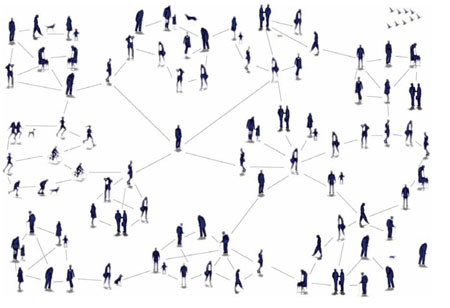
\includegraphics[width=.99\textwidth]{sixdegrees.png}
    \end{column}
  \end{columns}
}

\frame{
  \frametitle{The idea of the Small World Effect}

  Frigyes Karinthy first introduced this idea in his 1929 short story
  \emph{Chains}.
  \pause

  \vspace{0.5cm}
  In the 1960s the small world experiment (Stanley Milgram et al.) formalised
  the aforementioned concept.
  \pause

  \vspace{0.5cm}
  It confirmed the average distance of $6$ and resulted in
  general awareness of the \emph{small world effect}.
  \pause

  \hspace{0.5cm} $\to$ the \emph{average distance} linking two nodes of the same
  network can be \emph{orders of magnitude} smaller than the number of nodes the
  network actually has.
}


\frame{
  \frametitle{Small World Network Characteristics}

  Mathematically speaking, a small world network has the following properties:
  \pause

  \begin{itemize}
    \item Low average path length (distance).
    \pause
    \item High clustering coefficient.
    \pause
    \item Scale-free degree distribution.
  \end{itemize}
}

\frame{
  \frametitle{SWNs' characteristics insight}

  The \emph{distance} between two nodes in a graph is the minimum number of
  edges to be traversed in order to get from the first node to the second.
  \pause

  \vspace{0.5cm}
  \emph{Clustering} is the tendency of real networks to form \emph{cliques}
  (i.e. subsets of nodes in which all nodes are connected to each other).
  \pause

  \vspace{0.5cm}
  \emph{Scale-free} networks have a node degree distribution which follows a
  power law:

  \[ P(k) \sim k^{-\gamma} \hspace{1.2cm} 
\includegraphics[width=20mm, height=10mm]{angry.png} \]
}

\frame{\frametitle{More about scale-free networks}
\vspace{0.1cm}
Actually, this is not as hard as it seems!
\hspace{0.3cm} 
\includegraphics[width=7mm,height=7mm]{happy.png}

\vspace{0.3cm}
Check this out!
\vspace{0.1cm}
\begin{figure}[ht!]
  \centering
  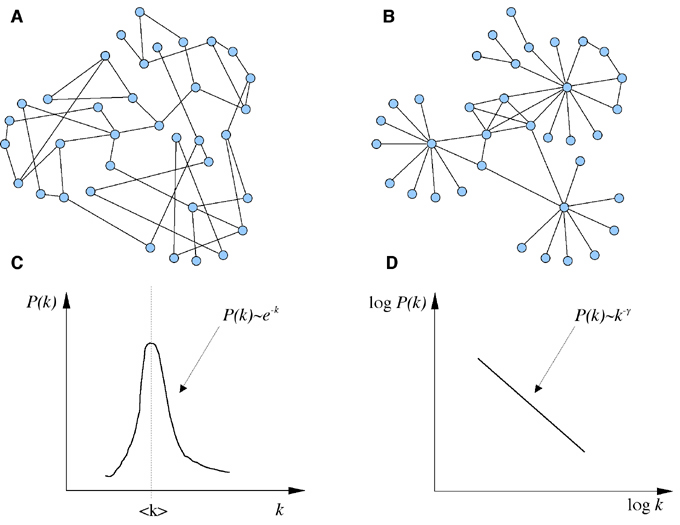
\includegraphics[height=40mm,width=60mm]{sfnet.png}
  \caption*{Comparison between random and scale-free networks}
\end{figure}
}

\frame{\frametitle{Real World applications of SWNs}

\begin{columns}

\begin{column}[T]{0.3\textwidth}

\begin{figure}[ht!]
  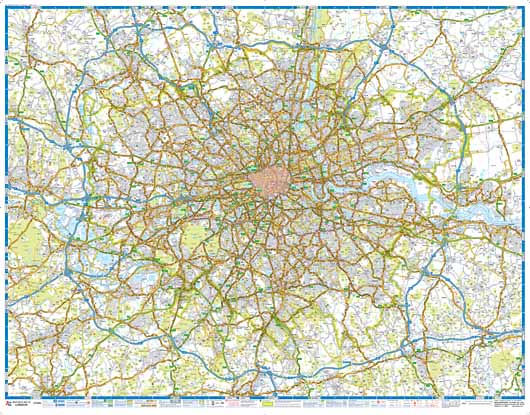
\includegraphics[width=30mm,height=30mm]{roadmap.png}
  \caption*{London Road Map}
\end{figure}

\end{column}

\begin{column}[T]{0.3\textwidth}

\begin{figure}[ht!]
 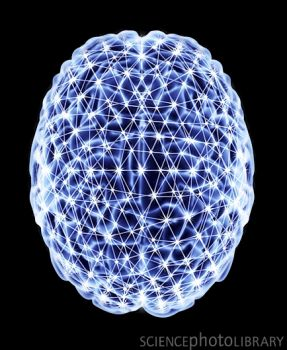
\includegraphics[width=30mm,height=30mm]{neuralnets.png}
\caption*{Neural networks}
\end{figure}

\end{column}

\begin{column}[T]{0.3\textwidth}

\begin{figure}[ht!]
 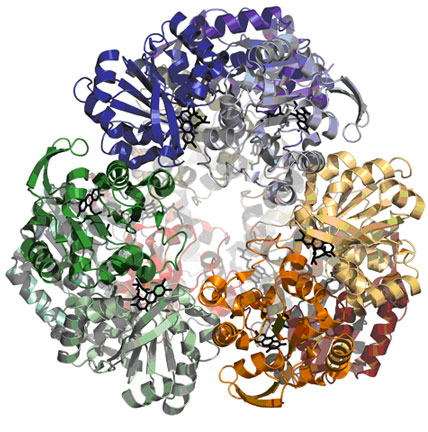
\includegraphics[width=30mm,height=30mm]{proteinstruct.png}
\caption*{Protein Structure}
\end{figure}

\end{column}

\end{columns}

}

\frame{\frametitle{Moving forward...}
By integrating existing generation algorithms and visualisations into a single,
easy-to-use interface, the user can make a head start into the large world of
small world networks.

\pause
\vspace{0.5cm}
So...let's check the \emph{algorithms} that help to the born of the small-world
networks' simulation...
}


\subsection{Generation Algorithm}

\frame{\frametitle{Erd\H{o}s-R\'{e}nyi}

\checklist{0}{0}{0}

\begin{columns}

\begin{column}[T]{.3\textwidth}
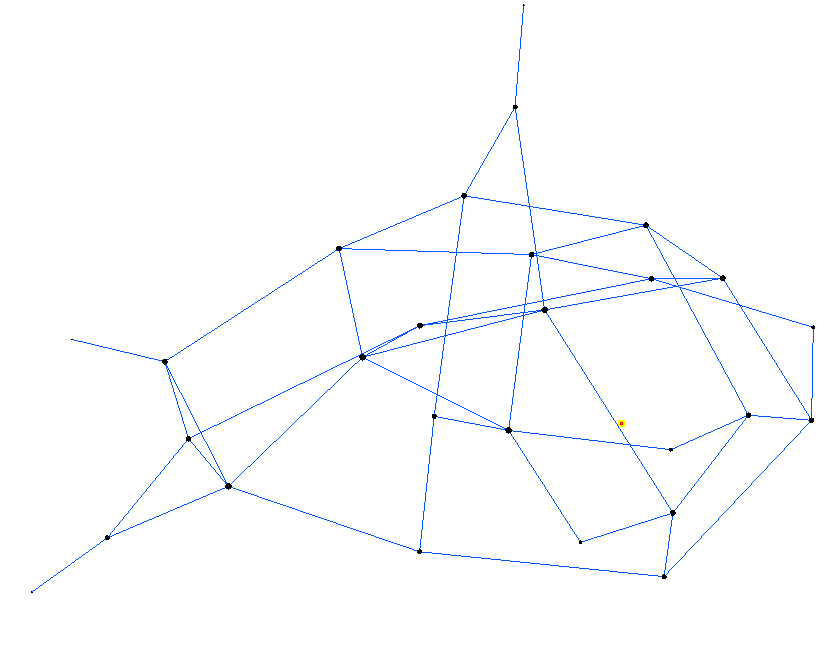
\includegraphics[height=30mm,width=30mm]{erdos.png}
\end{column}

\begin{column}[T]{.7\textwidth}

\begin{itemize}
  \item In the beginning there was Erd\H{o}s \dots and R\'{e}nyi
  \pause
  \item Random Graph
  \pause
  \item However \dots
  \pause
  \item No SWN properties

\end{itemize}
\end{column}
\end{columns}

}


\frame{\frametitle{Watts-Strogatz}

\checklist{1}{1}{0}

\begin{columns}

\begin{column}[T]{.3\textwidth}

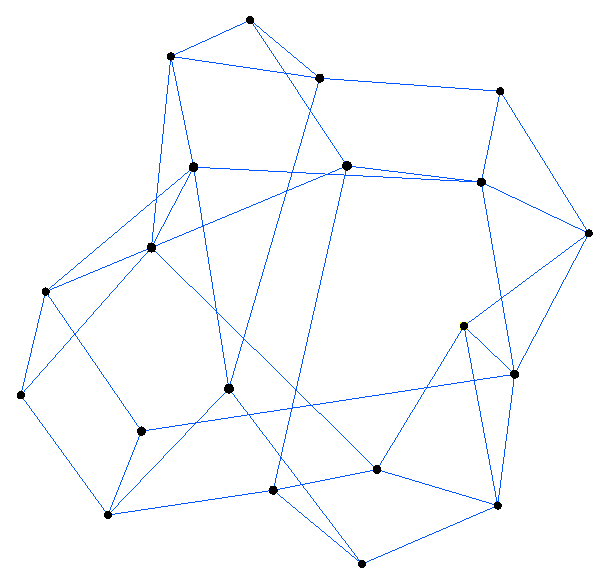
\includegraphics[height=30mm,width=30mm]{watts.png}

\end{column}

\begin{column}[T]{.7\textwidth}
\begin{itemize}
  \item Then in 1998 finally \dots Watts-Strogatz
  \pause
  \item Random graph
  \pause
  \item This time with SWN properties included! \dots
  \item Short average path and high clustering

\end{itemize}
\end{column}
\end{columns}
}

\frame{\frametitle{Barabasi-Albert}

\checklist{1}{0}{1}

\begin{columns}
\begin{column}[T]{.3\textwidth}

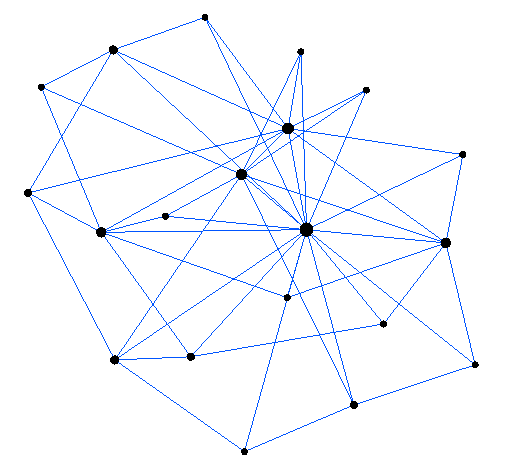
\includegraphics[height=30mm,width=30mm]{barabasi.png}

\end{column}

\begin{column}[T]{.7\textwidth}
\begin{itemize}
  \item It gets better!
  \pause
  \item The random graph is no more
  \pause
  \item Same amount of SWN properties included! \dots
  \item Scale free exponent and short average path

\end{itemize}
\end{column}
\end{columns}

}

\frame{\frametitle{Preferential attachment with clustering}

\checklist{1}{1}{1}

\begin{columns}

\begin{column}[T]{.3\textwidth}

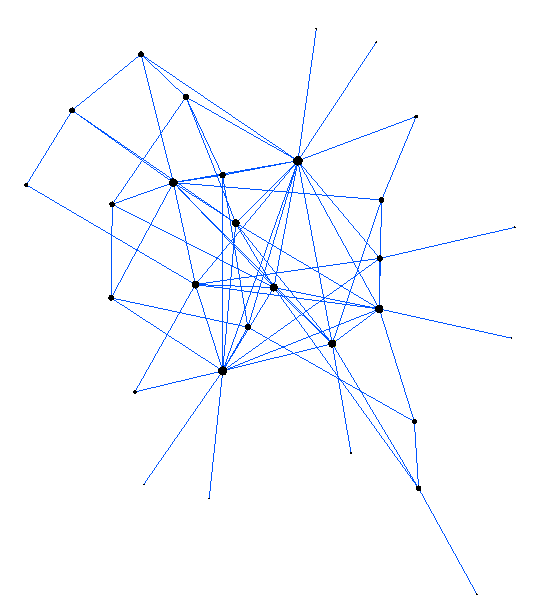
\includegraphics[height=30mm,width=30mm]{preferential.png}

\end{column}
\begin{column}[T]{.7\textwidth}


\begin{itemize}
  \item The future is here! Thanks to Imperial College
  \pause
  \item Similar to Barabasi-Albert but with clustering!
  \pause
  \item All SWN properties

\end{itemize}

\end{column}
\end{columns}

}

\frame{\frametitle{Bipartite}

\checklist{1}{1}{1}

\begin{columns}

\begin{column}[T]{.3\textwidth}

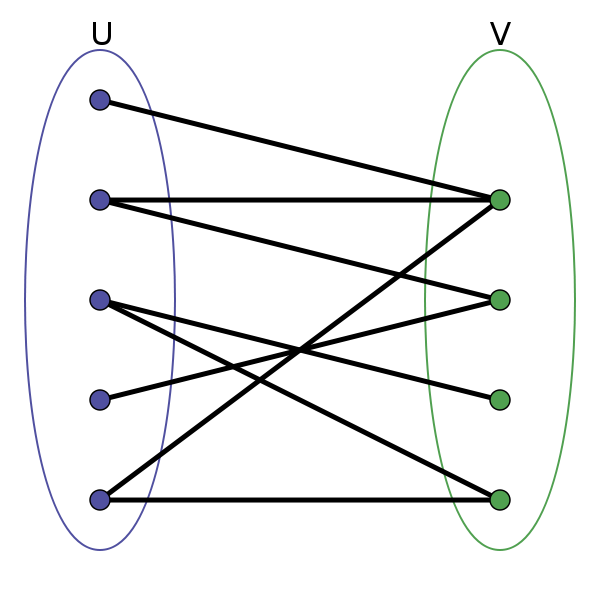
\includegraphics[height=30mm,width=30mm]{bipartite.png}

\end{column}
\begin{column}[T]{.7\textwidth}

\begin{itemize}
  \item The future is here! (again) Thanks to Imperial College
  \pause
  \item Completely different generation method.
  \pause
  \item All SWN properties

\end{itemize}

\end{column}
\end{columns}
}

\renewcommand{\ExtraText}{
\includegraphics[width=1cm]{dilbert.png}}
\section{Engineering}

\subsection{Qt}

\frame{\frametitle{Qt}

The Royal Road to desktop applications:
\ 
\includegraphics[width=.4cm]{qt.png}\\
\pause

Cross-platform. \pause
Open source. \pause
Awesome. \pause

\begin{itemize}
  \item widgets \Therefore native look and feel \pause
  \item \texttt{stdlib} replacement \Therefore Oh, look: a sane
    \texttt{string} class \pause
  \item modern C++ (signals, introspection) \Therefore Loose
    coupling. Better overall design. \pause
  \item threading/concurrency \Therefore \textsc{speed} \pause
  \item networking, XML support, OAuth library \Therefore Less
    hassle. More features.
\end{itemize}
\pause

Oh, and it's cross-platform.
\pause
Same code: Linux, Windows, OSX.

}

\subsection{Graph drawing}

\frame{
  \frametitle{Graph drawing}

  Graph drawing is hard for humans... \pause and harder for computers:

  \begin{itemize}
    \pause
    \item Non-formal requirements (human taste)
    \pause
    \item Should adapt to a variety of different graphs
    \pause
    \item Should be fast
  \end{itemize}
}

\frame{
  \frametitle{Force-directed algorithms}

  For Visigoth, we use an optimized ``force directed'' algorithm.
  \pause

  Each node is a charged particle, and each edge is a rubber band.
  \pause

  \vspace{0.5cm}
  We chose this kind of algorithm because:

  \begin{itemize}
    \item It gives good results for most graphs
    \pause
    \item It is easy to implement, few tens of lines of \emph{C++}
      (\emph{C++}!) in our case
    \pause
    \item We can show the stabilization in real time (bling)
  \end{itemize}

}

\subsection{FADE}

\frame{
  \frametitle{FADE}

  However, it also is... \pause slow.\\
  Quite slow: $O(n^2)$, where $n$ is the number of nodes.
  \pause

  \vspace{0.5cm}
  The solution? FADE, an algorithm that achieves speed through approximation.
}

\frame{
  \frametitle{TreeCodes}

  FADE works by storing the nodes of a \emph{TreeCode}, a data structure that
  stores the nodes while recursively subdividing the space:
  \pause

  \begin{columns}
    \begin{column}{0.5\textwidth}
      \centering
      \begin{tikzpicture}[y=0.80pt, x=0.8pt,yscale=-0.3, xscale=0.3, inner sep=0pt, outer sep=0pt]
  \path[draw=black,line join=miter,line cap=butt,line width=0.800pt]
  (356.4286,94.5050) -- (356.4286,598.7908);
  \path[draw=black,line join=miter,line cap=butt,line width=0.800pt]
  (102.1429,348.7908) -- (605.7143,348.7908);
  \path[draw=black,line join=miter,line cap=butt,line width=0.800pt]
  (102.1429,220.2193) -- (607.1429,220.2193);
  \path[draw=black,line join=miter,line cap=butt,line width=0.800pt]
  (229.2857,93.0765) -- (229.2857,598.7908);
  \path[draw=black,line join=miter,line cap=butt,line width=0.800pt]
  (485.0000,93.7908) -- (485.0000,349.5050);
  \path[draw=black,line join=miter,line cap=butt,line width=0.800pt]
  (101.4286,477.3622) -- (356.4286,477.3622);
  \path[draw=black,line join=miter,line cap=butt,line width=0.800pt]
  (420.7143,220.2193) -- (420.7143,349.5050);
  \path[draw=black,line join=miter,line cap=butt,line width=0.800pt]
  (356.4286,285.2193) -- (485.0000,285.2193);
  \path[draw=black,line join=miter,line cap=butt,line width=0.800pt]
  (292.1429,348.0765) -- (292.1429,476.6479);
  \path[draw=black,line join=miter,line cap=butt,line width=0.800pt]
  (228.5714,413.0765) -- (357.1429,413.0765);
  \path[draw=black,line join=miter,line cap=butt,line width=0.800pt]
  (165.7143,477.3622) -- (165.7143,599.5050);
  \path[draw=black,line join=miter,line cap=butt,line width=0.800pt]
  (100.7143,540.9336) -- (229.2857,540.9336);
  \path[cm={{0.86607143,0.0,0.0,0.86607143,(-133.53636,-75.700851)}},draw=black,fill=c7372ff]
  (506.4286,453.4336)arc(0.000:180.000:7.500)arc(-180.000:0.000:7.500) -- cycle;
  \path[cm={{0.86607143,0.0,0.0,0.86607143,(-280.6792,-62.843726)}},draw=black,fill=c7372ff]
  (506.4286,453.4336)arc(0.000:180.000:7.500)arc(-180.000:0.000:7.500) -- cycle;
  \path[cm={{0.86607143,0.0,0.0,0.86607143,(-185.6792,29.656274)}},draw=black,fill=c7372ff]
  (506.4286,453.4336)arc(0.000:180.000:7.500)arc(-180.000:0.000:7.500) -- cycle;
  \path[cm={{0.86607143,0.0,0.0,0.86607143,(-180.6792,75.013418)}},draw=black,fill=c7372ff]
  (506.4286,453.4336)arc(0.000:180.000:7.500)arc(-180.000:0.000:7.500) -- cycle;
  \path[cm={{0.86607143,0.0,0.0,0.86607143,(-291.75062,136.79913)}},draw=black,fill=c7372ff]
  (506.4286,453.4336)arc(0.000:180.000:7.500)arc(-180.000:0.000:7.500) -- cycle;
  \path[cm={{0.86607143,0.0,0.0,0.86607143,(-254.25063,184.65628)}},draw=black,fill=c7372ff]
  (506.4286,453.4336)arc(0.000:180.000:7.500)arc(-180.000:0.000:7.500) -- cycle;
  \path[cm={{0.86607143,0.0,0.0,0.86607143,(102.53509,22.87056)}},draw=black,fill=c7372ff]
  (506.4286,453.4336)arc(0.000:180.000:7.500)arc(-180.000:0.000:7.500) -- cycle;
  \path[cm={{0.86607143,0.0,0.0,0.86607143,(21.463659,-64.272297)}},draw=black,fill=c7372ff]
  (506.4286,453.4336)arc(0.000:180.000:7.500)arc(-180.000:0.000:7.500) -- cycle;
  \path[cm={{0.86607143,0.0,0.0,0.86607143,(23.249374,-116.41515)}},draw=black,fill=c7372ff]
  (506.4286,453.4336)arc(0.000:180.000:7.500)arc(-180.000:0.000:7.500) -- cycle;
  \path[cm={{0.86607143,0.0,0.0,0.86607143,(1.4636592,-155.70087)}},draw=black,fill=c7372ff]
  (506.4286,453.4336)arc(0.000:180.000:7.500)arc(-180.000:0.000:7.500) -- cycle;
  \path[fill=black] (160.31509,332.78058) node[above right] (text6462) {\tiny{1}};
  \path[fill=black] (307.43341,319.70856) node[above right] (text6462-4) {\tiny{2}};
  \path[fill=black] (441.40405,239.94313) node[above right] (text6462-9) {\tiny{3}};
  \path[fill=black] (465.61832,280.30029) node[above right] (text6462-98) {\tiny{4}};
  \path[fill=black] (463.73944,332.14725) node[above right] (text6462-5) {\tiny{5}};
  \path[fill=black] (255.68974,433.98373) node[above right] (text6462-0) {\tiny{6}};
  \path[fill=black] (260.68976,470.65741) node[above right] (text6462-7) {\tiny{7}};
  \path[fill=black] (143.21951,522.34161) node[above right] (text6462-3) {\tiny{8}};
  \path[fill=black] (186.40405,580.65741) node[above right] (text6462-43) {\tiny{9}};
  \path[fill=black] (542.83264,419.586) node[above right] (text6462-02) {\tiny{10}};
  \path[draw=black,line join=miter,line cap=butt,line width=0.800pt]
  (606.0915,92.7173) -- (606.0915,599.8138) -- (100.0051,599.8138) --
  (100.0051,92.7173);
  \path[draw=black,line join=miter,line cap=butt,line width=0.800pt]
  (100.0051,93.7274) -- (605.0814,93.7274);
\end{tikzpicture}

    \end{column}

    \pause

    \begin{column}{0.5\textwidth}
      \centering
      \begin{tikzpicture}[yscale=0.8, xscale=0.8, grow cyclic]
  \node {\square}
  child {
    node {\square}
    child {
      node {\square}
      child {node {\footnotesize{1}}}
    }
    child {
      node {\square}
      child {node {\footnotesize{2}}}
    }
  }
  child {
    node {\square}
    child {
      node {\square}
      child {
        node {\square}
        child { node{\footnotesize{3}} }
        child { node{\footnotesize{4}} }
      }
      child {
        node {\square}
        child {node{\footnotesize{5}}}
      }
    }
  }
  child {
    node {\square}
    child {
      node {\square}
      child {
        node {\square}
        child {node{\footnotesize{6}}}
        child {node{\footnotesize{7}}}
      }
    }
    child {
      node {\square}
      child {
        node {\square}
        child {node{\footnotesize{8}}}
      }
      child {
        node {\square}
        child {node{\footnotesize{9}}}
      }
    }
  }
  child {
    node {\square}
    child { node {\footnotesize{10}} }
  }
  ;
\end{tikzpicture}

    \end{column}
  \end{columns}
}

\frame{
  \frametitle{FADE}
  In our case, the \emph{TreeCode} subdivides the space recursively in 8 cubes.

  Once the \emph{TreeCode} is ready, when calculating the repulsion forces for
  each node:

  \begin{itemize}
    \pause
    \item Pick a cube in the \emph{TreeCode}
    \pause
    \item If the cube is ``far enough'', it will be treated as a single
      node, and the repulsion calculated based on how many nodes it contains
    \pause
    \item Otherwise, subdivide the cube, and try again with the 8 ``children''
      cubes.
  \end{itemize}
}

\subsection{C++}

\frame{
  \frametitle{C++}

  \emph{C++}, the world's friendliest language...
  \pause

  If you like segfaults.
  \pause

  And 3-pages long compiler errors.
}

\frame{
  \frametitle{C++}

  We chose \emph{C++} because of \emph{Qt}, but some team members were scared.

  However, it does have its advantages, and it served us well:

  \begin{itemize}
    \pause
    \item Tools: Mainly \emph{Qt} and \emph{OpenGL}
    \pause
    \item Performance: ours is a CPU bound application, and with \emph{C++} we
      can squeeze our machines more, especially with manual memory management.
    \pause
    \item Abstraction: while \emph{C} and \emph{C++} are both fast and popular,
      doing O-O in \emph{C} is \textbf{not} nice (take a look at
      GObject\footnote{\url{http://developer.gnome.org/gobject/}} for details).
  \end{itemize}
}

\frame{
  \frametitle{C++, the dark side}

  But...

  \begin{itemize}
    \pause
    \item Unmanaged memory is not nice, most of the times. Memory leaks are not
      nice. Segfaults are not nice.
    \pause
    \item The language is a mess. Too much stuff in too little space: templates,
      overloading, friends\dots\\
      \pause
      {\tiny \lstinputlisting{cpperr}}
  \end{itemize}
  \pause
  In any case, we are happy with our choice, and we don't care what
  the haters say.
}



\subsection{OpenGL}

\frame{
  \frametitle{OpenGL}

  OpenGL $\to$ super fast graphics with hardware acceleration!
  \pause

  \vspace{0.5cm}
  We can...

  \begin{itemize}
    \pause
    \item Pan left/right/up/down
    \pause
    \item Zoom in/out.
    \pause
    \item And do it all in 3D - real-time!
  \end{itemize}
  \pause

  \vspace{0.5cm}
  Thanks to the FADE optimisation, it's fast - 1000s of nodes.
}

\frame{
  \frametitle{OpenGL selection}
  Selection made easy...
  \pause

  \vspace{0.5cm}
  It's now the same for 2D and 3D:

  OpenGL ``unprojects'' the mouse click.
  \pause

  \vspace{0.5cm}
  Selection triggers node stats recalculation, colouring...
}




\section{DEMO}

\section{Conclusion}

\frame{
  \frametitle{Looking back, and forward}
  We enjoyed coding Visigoth, we hope you'll enjoy playing with it.

  While sometimes lacking in verification, we constantly delivered. We
  even proposed a lot of features of our own!

  And it's not over, more are coming soon:
  \begin{itemize}
    \pause
    \item Multi-threaded and even faster engine
    \pause
    \item Game based on small-world networks
    \pause
    \item Graph generation scriptable by the user via \emph{JavaScript}
  \end{itemize}

  \pause

  And who knows what else\dots
}

\frame{

\begin{center}
  \Huge Questions?
\end{center}
}

\end{document}
